\documentclass[../main.tex]{subfiles}
\graphicspath{{\subfix{../figures/}}}

\begin{document}
\chapter{Hardware Integration} \label{chap:hw}
This chapter contains preliminary steps for integrating a trained agent into UWG5's microcontroller unit (MCU). Although a fully functional device is not our target, we must prepare a solution to four practical problems that might arise in the next prototype phase.

\section{Model Quantization}
Model quantization is a technique used in machine learning to reduce the memory footprint and computational requirements of a model, typically deep learning models, without significantly sacrificing their performance \cite{soumyad23,rishi2024}. By representing their weights in low-precision data types (such as 8-bit integers, aka. INT8), quantization achieves the following benefits:
\begin{enumerate}
    \item \textbf{Memory efficiency}: quantization reduces the memory needed to store model parameters. Smaller model sizes are crucial for deploying models on resource-constrained devices, edge devices, or cloud servers.
    \item \textbf{Inference speed}: lower-precision representations allow faster computations during inference. Reduced precision means fewer bits to process, leading to quicker predictions.
    \item \textbf{Energy saving}: quicker computation consumes less energy, which is critical for many embedded applications like drones or mobile robots.
\end{enumerate}
However, quantization introduces challenges, especially with much lower precision, like INT8, which has a very limited dynamic range. Fine-tuning and balancing accuracy with model size reduction are essential considerations.

As introduced in the first chapter, UWG5 thermostats use STM32L452 MCU from ST Microelectronics. Arm® Cortex®-M4 32-bit operates this ultra-low-power series with a floating-point unit (FPU) and offers up to 512KB Flash and 160KB SRAM. Fortunately, it also supports the CMSIS DSP (Digital Signal Processing) package for handling heavy computing tasks, including sensor signal processing and deep learning inference. Thus, the optimal data type for my model after quantization is
\begin{equation}
    \text{single node size} = \floor*{\frac{512 - 110}{67,841}} = \text{32 bit}
\end{equation}
\begin{multicols}{2}
    \begin{itemize}
        \item 512 (KB) total on-board memory size
        \item 110 (KB) UWG5's firmware size
        \item 67,841 nodes of actor's network
    \end{itemize}
\end{multicols}


\section{Sensor Fusion for Missing Feedback}
Connection loss due to physical disturbances occurs often (Fig. \ref{fig:conn_loss}). They might originate from high-frequency converters of a ventilator's AC motors, long USB cables, or sudden power shortages, which result in Not-A-Number (NAN) values (Fig. \ref{fig:missing_fb}).
\begin{figure}[htbp]
\centering
\begin{subfigure}{\textwidth}
    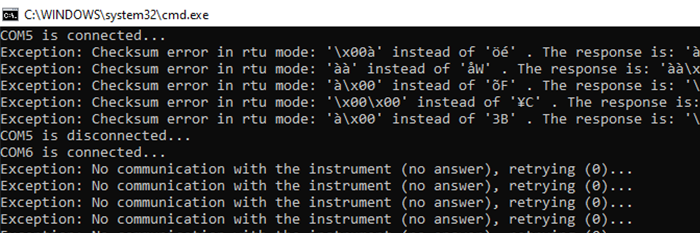
\includegraphics[width=\linewidth]{figures/conn_loss.png}
    \caption{Missing feedback due to unstable connection}
    \label{fig:conn_loss}
\end{subfigure}
\begin{subfigure}{\textwidth}
    \includegraphics[width=\linewidth]{figures/missing_fb.png}
    \caption{Missing feedback due to unstable connection}
    \label{fig:missing_fb}
\end{subfigure}
\end{figure}

All datasets in chapter \ref{chap:intro} face this issue. Yet, I could remove the missing values as they were unimportant. Doing so is no longer valid in operation, as controllers must always get feedback. I resolve this issue with sensor fusion using a "linear minimum mean squared error" (LMMSE) estimator. The core idea is that when one sensor goes blank, the others still provide us with sufficient information to estimate it. As its name suggests, LMMSE is the best linear estimator regarding mean-squared error for any system, as long as noises are Gaussian. It is also easy to implement and memory-efficient due to its recursive nature (Alg. \ref{alg:lmmse}).

Afterwards, the missing spots in figure \ref{fig:missing_fb} are now filled in as
\begin{figure}
    \centering
    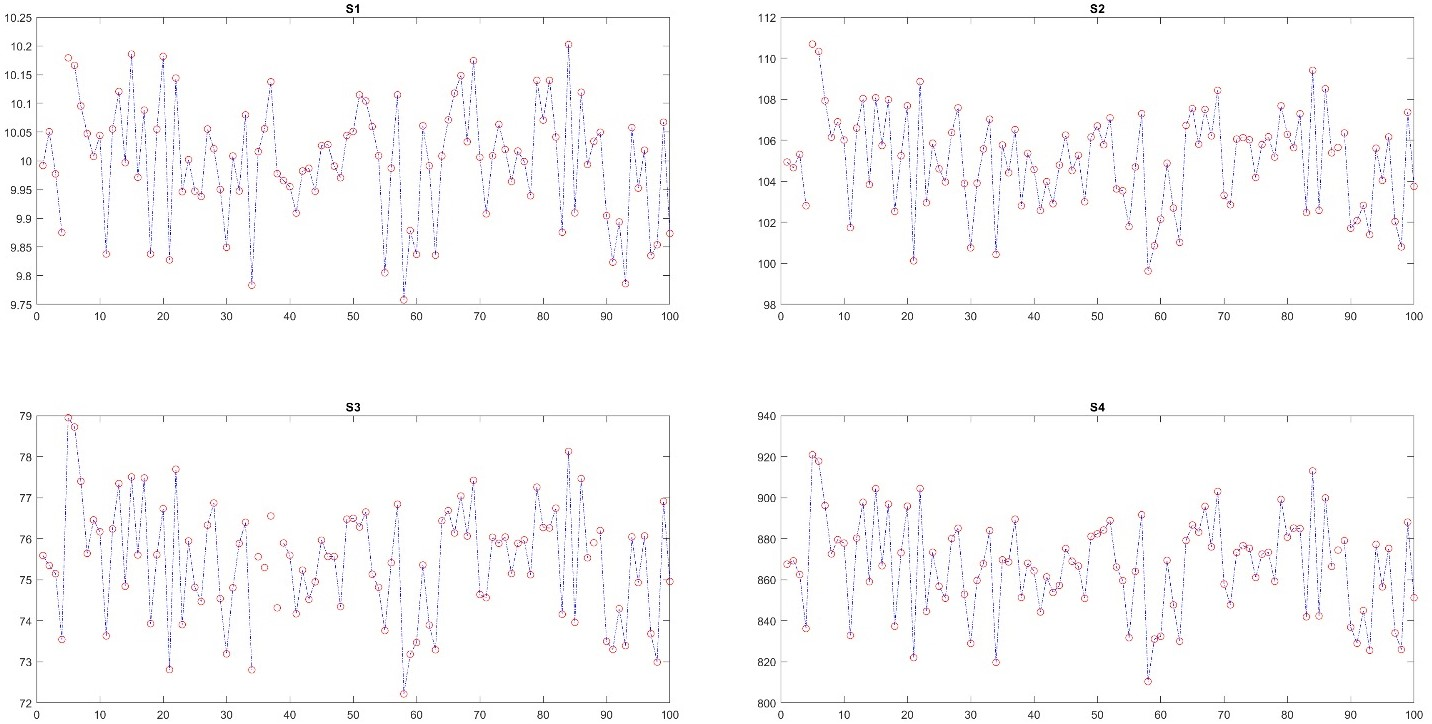
\includegraphics[width=1\linewidth]{figures/lmmse.jpg}
    \caption{LMMSE fills in empty gaps}
    \label{fig:lmmse}
\end{figure}
\todo{update figs + pseud-code}

\nomenclature[D]{sensor fusion}{combine data from various sensors to provide a better estimate}
\nomenclature[D]{IID}{Independent and Identical Distribution, a stochastic process in which samples are independent and have an identical distribution for all time steps}
\nomenclature[D]{MLE}{Maximum Likelihood, a statistical method used to estimate unknown parameters by maximizing the probability of observing recorded data}
\nomenclature[D]{MAP}{Maximum A Posteriori, a statistical method based on Bayesian theorem, used to estimate unknown parameters by maximizing the posterior distribution of available observations}
\nomenclature[D]{MMSE}{Minimum Mean Squared Error, a statistical estimator based on Bayesian theorem, used to estimate unknown parameters by minimizing the mean squared error. People often use a linear version for simplicity (LMMSE). When the model is linear and the noises are Gaussian, LMMSE and MAP are identical.}
\nomenclature[D]{LMMSE}{See \textbf{MMSE}.}

\section{Fault Detection}
This section shows the sequence diagram and state machine

\section{Fault Recovery}

\section{Processor-in-the-Loop Testing}
Processor-in-the-loop (PIL) testing is a crucial technique in the model-based development framework. It involves running software models (Simulink) on a target hardware platform (STM32L452 MCU) to verify their behavior. PIL testing ensures that our model behaves correctly when executed on any real-world target. With this early validation process, engineers can detect issues related to code generation, timing, and hardware interactions.

\end{document}
